% --------------------------------------------------------------
% This is all preamble stuff that you don't have to worry about.
% Head down to where it says "Start here"
% --------------------------------------------------------------
 
\documentclass[12pt]{article}
 
\usepackage[margin=1in]{geometry} 
\usepackage{amsmath,amsthm,amssymb,scrextend}
\usepackage{fancyhdr}
\usepackage{enumitem}
\usepackage{amsmath}
\usepackage{amssymb}
\usepackage{textcomp}
\usepackage{fancybox}
\usepackage{tikz}
\usepackage{tasks}
\pagestyle{fancy}
\usepackage[makeroom]{cancel}
\usepackage{graphicx}
\usepackage{caption}
\usepackage{mwe}
\usepackage{tikz}
\usetikzlibrary{positioning}

\newcommand{\N}{\mathbb{N}}
\newcommand{\Z}{\mathbb{Z}}
\newcommand{\I}{\mathbb{I}}
\newcommand{\R}{\mathbb{R}}
\newcommand{\Q}{\mathbb{Q}}
\renewcommand{\qed}{\hfill$\blacksquare$}
\let\newproof\proof
\renewenvironment{proof}{\begin{addmargin}[1em]{0em}\begin{newproof}}{\end{newproof}\end{addmargin}\qed}
% \newcommand{\expl}[1]{\text{\hfill[#1]}$}
 
\newenvironment{theorem}[2][Theorem]{\begin{trivlist}
\item[\hskip \labelsep {\bfseries #1}\hskip \labelsep {\bfseries #2.}]}{\end{trivlist}}
\newenvironment{lemma}[2][Lemma]{\begin{trivlist}
\item[\hskip \labelsep {\bfseries #1}\hskip \labelsep {\bfseries #2.}]}{\end{trivlist}}
\newenvironment{problem}[2][Problem]{\begin{trivlist}
\item[\hskip \labelsep {\bfseries #1}\hskip \labelsep {\bfseries #2.}]}{\end{trivlist}}
\newenvironment{exercise}[2][Exercise]{\begin{trivlist}
\item[\hskip \labelsep {\bfseries #1}\hskip \labelsep {\bfseries #2.}]}{\end{trivlist}}
\newenvironment{reflection}[2][Reflection]{\begin{trivlist}
\item[\hskip \labelsep {\bfseries #1}\hskip \labelsep {\bfseries #2.}]}{\end{trivlist}}
\newenvironment{proposition}[2][Proposition]{\begin{trivlist}
\item[\hskip \labelsep {\bfseries #1}\hskip \labelsep {\bfseries #2.}]}{\end{trivlist}}
\newenvironment{corollary}[2][Corollary]{\begin{trivlist}
\item[\hskip \labelsep {\bfseries #1}\hskip \labelsep {\bfseries #2.}]}{\end{trivlist}}
 
\setlength{\parindent}{0pt}
\begin{document}
 \settasks{
	counter-format=(tsk[r]),
	label-width=4ex
}
% --------------------------------------------------------------
%                         Start here
% --------------------------------------------------------------

\lhead{Math 475}
\chead{Homework 3}
\rhead{Meenmo Kang}

\begin{enumerate}
    \item[\bf 3.4.3] Generalize Application 5 by choosing (how many?) integers from the set \{1,2,...,2n\}.
    
    \vspace{0.1\baselineskip}
    \textbf{\textit{Application 5 }}Given 101 integers from 1, 2, . . . , 200, there are at least two integers such that one of them is divisible by the other.\\
    
    Suppose all numbers in the set are factored out as many 2's as possible. Then all numbers are expressed in the form $2^a\cdot b$, where $a\ge 0$ and $b$ is odd. The number of odd integers in this set is $n$, while $n+1$ integers (instead of 101) are chosen. In other words, we choose $n+1$ integers from the set like
    $$2^{a_1}b_1,\; 2^{a_2}b_2,\;\ldots\;, 2^{a_{n+1}}b_{n+1}$$
    Consider the number of odd integers, $n$, in this set to be pigeonholes and $b_i|_{i=1}^{n+1}$ to be pigeons. Since there are more pigeons than pigeonholes, there are at least two identical $b_i,\;b_j$. This implies that one integer can be divided by the other integers. \\
    
    \item[\bf 3.4.5] Show that if n + 1 distinct integers are chosen from the set \{l, 2, ... , 3n\}, then there are always two which differ by at most 2.\\
    \begin{itemize}
        \item Pigeon: each integer from 1 to 3n
        \item Pigeonholes: Each partition \{1, 2, 3\},\{4, 5, 6\}, ... , \{2n-2, 2n-1, 2n\}
    \end{itemize}
    Even if we sample one number each from each partition, at least two numbers have to be sampled from a same partition whose difference is at most 2 when sampling n+1 distinct integers.\\
    
    \item[\bf 3.4.8] Use the pigeonhole principle to prove that the decimal expansion of a rational number $m/n$ eventually is repeating. For example,
    $$\frac{34,478}{99,900} = 0.34512512512512512\ldots .$$\\
    
    Without loss of generality, suppose $m$ and $n$ are positive integers and it is given that $m/n$ is repeating eventually. Let $q$ be the quotient of this division and $r_0$ be the remainder. $$m=qn+d_0$$
    By multiplying 10 by $r_0$, we can derive
    $$10r_0 = q_1n + r_1$$
    And this equation can be generalized.
    $$10r_{i-1}=q_in+r_i$$
    Note that $\{r_i\}$ is an infinite sequence and $1\le r_1 \le n-1$ since this is remainder after dividing by $n$. Thus there must be at least a pair $r_i=r_j$ by the Pigeonhole Principal.
    \item[\bf 3.4.9] In a room there are 10 people, none of whom are older than 60 (ages are given in whole numbers only) but each of whom is at least 1 year old. 
    
    \begin{itemize}
        \item Prove that we can always find two groups of people (with no common person) the sum of whose ages is the same.
        \begin{itemize}
            \item The maximum sum of group age: $\sum\limits_{i=51}^{60} i = 555$
            \item The minimum sum of group age  $\sum\limits_{i=1}^{10} = 55$
            \item The number of possible age sums = 555-55+1 = 501
        \end{itemize}
        
        \vspace{2\baselineskip}
        \begin{itemize}
            \item Pigeon: $2^{10} - 1 = 1023$ \hfill (without empty set)
            \item Pigeon holes: 501
        \end{itemize}
        
        By Pigeonhole theorem, it is always possible to find two groups of people that have the same age sum.\\
        
        \item Can 10 be replaced by a smaller number?\\
        
        Yes. As long as the number of pigeon is bigger than pigeonholes, it is okay. For this case, even if there are only 9 people in the room, it is still possible to find two groups of people that have the same age sum since $2^9-1$ = 511.\\
        
    \end{itemize}
     
    

    \item[\bf 3.4.10] A child watches TV at least one hour each day for seven weeks but, because of parental rules, never more than 11 hours in anyone week. Prove that there is some period of consecutive days in which the child watches exactly 20 hours of TV. (It is assumed that the child watches TV for a whole number of hours each day.)\\
    
    Let $t_i$ be the total amount of time the child has watched from the first day up to $ith$ day and $d_i$ be the amount of time the child watched in $ith$ day. 
    $$t_i = d_1+d_2+\ldots+d_i$$
    Since the child is not allowed to watch TV no more than 11 hours per week, we can formulate as below.
    $$1\le t_1\le t_2\le\ldots\le t_{49}\le 77$$
    Let us add by 20 to every term above.
    $$21\le 20+t_1\le 20+t_2\le\ldots\le 20+t_{49}\le 97$$
    
    So, there are 98 integers in total: $t_1\; ...\; t_{49}$ and $20+t_1\; ...\; 20+t_{49}$. Since the range of integers between 1 and 97, there must be at least two identical integer. But they are not in a certain group as both groups are increasing sequence. In other words, this number has to be one from each group, like
    $$t_i = t_j + 20 \Leftrightarrow (d_1+...+d_{i}) - (d_1+...+d_j) = d_{j+1}+...+d_i = 20$$\\
    
    \item[\bf 3.4.14] A bag contains 100 apples, 100 bananas, 100 oranges, and 100 pears. If I pick one piece of fruit out of the bag every minute, how long will it be before I am assured of having picked at least a dozen pieces of fruit of the same kind?\\
    
    Consider the extreme case: I sample 44 fruits, but they were each kind of 11 pieces. Therefore, at least 45 fruits have to be picked in order to make sure at least a dozen pieces of fruit of the same kind have been chosen.\\
    
    \item[\bf 3.4.16] Prove that in a group of $n > 1$ people there are two who have the same number of acquaintances in the group. (It is assumed that no one is acquainted with oneself. )\\
    
    A person in the group may know no one in the group or know everyone, at most $n-1$ people except for me. However, we assume that acquaintances are mutual. i.e. if someone knows $n-1$ people, everyone else in the group have at least 1 acquaintance. Or, if someone does not have any acquaintance in the group, then other people in the group would have at most $n-2$ acquaintances. Hence, there are $n-1$ possible number of acquaintances people have. Consider this to be pigeonholes of the Pigeonhole Principal and the number of people $n$ to be pigeons. Since there are more pigeons than pigeonholes, there must be two people who have the same number of acquaintances in the group.\\
    
    \item[\bf 3.4.18] Prove that of any five points chosen within a square of side length 2, there are two whose distance apart is at most $\sqrt{2}$.\\
    
    \begin{center}
        \tikzset{every picture/.style={line width=0.75pt}} %set default line width to 0.75pt     
        
        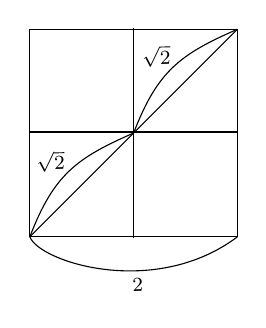
\begin{tikzpicture}[x=0.75pt,y=0.75pt,yscale=-1,xscale=1]
        %uncomment if require: \path (0,541.6666564941406); %set diagram left start at 0, and has height of 541.6666564941406
        
        %Shape: Rectangle [id:dp23102956138766606] 
        \draw   (110,280) -- (210,280) -- (210,380) -- (110,380) -- cycle ;
        %Straight Lines [id:da16555745351128492] 
        \draw    (160,279.5) -- (160,380.5) ;
        
        
        %Straight Lines [id:da7212596793995814] 
        \draw    (110,329.5) -- (210,329.5) ;
        
        
        %Straight Lines [id:da5582242533161783] 
        \draw    (110,380) -- (210,280) ;
        
        
        %Curve Lines [id:da5717057412991984] 
        \draw    (110,380) .. controls (114.5,392) and (170,410) .. (210,380) ;
        
        
        %Curve Lines [id:da47681696246506755] 
        \draw    (110,380) .. controls (121.5,350) and (132.5,342) .. (160,330) ;
        
        
        %Curve Lines [id:da7226416765910546] 
        \draw    (160,330) .. controls (171.5,300) and (182.5,292) .. (210,280) ;
        
        
        
        % Text Node
        \draw (120,344) node [scale=0.9,rotate=-358.41] [align=left] {{\footnotesize $\sqrt{2}$}};
        % Text Node
        \draw (171,293) node [scale=0.9,rotate=-358.41] [align=left] {{\footnotesize $\sqrt{2}$}};
        % Text Node
        \draw (162,403) node [scale=0.9,rotate=-358.41] [align=left] {{\footnotesize $2$}};
        \end{tikzpicture}
    \end{center}
    
    Let us divide this square into four squares with the length of side 1. Even if first four points are located on each distinct square, the fifth point has to be one of four squares. So, the distance of those two points within the same square would be lesser than $\sqrt{2}$.
    
    \item[\bf 3.4.20] Prove that $r(3, 3, 3) \le 17$.\\
    
    Pick a vertex of $K_{17}$ which is of three colours. Let us these colour to be red, green, and blue. By pigeonhole principal, there must be six edges with identical colour among 16 edges; say this colour to be red. The other end of each six edges is connected with either the other green or non-green edges. We can consider this to be $r(3,3)=6\le 17$.
\end{enumerate}
\end{document}